\documentclass[11pt,a4paper,landscape]{article}
\usepackage[margin=14mm,headheight=14pt,headsep=5mm,footskip=8mm]{geometry}
\usepackage[T1]{fontenc}
\usepackage{lmodern,microtype,xcolor,tikz,tabularx,booktabs,array,fancyhdr,hyperref,amsmath}
\usetikzlibrary{arrows.meta,positioning,calc}
\renewcommand{\familydefault}{\sfdefault}
\definecolor{navy}{HTML}{183447}
\definecolor{teal}{HTML}{147B80}
\definecolor{blue}{HTML}{226B9A}
\definecolor{orange}{HTML}{BA6425}
\definecolor{pale}{HTML}{EDF6F5}
\definecolor{paleblue}{HTML}{EDF3FA}
\definecolor{paleorange}{HTML}{FCF2E8}
\definecolor{slate}{HTML}{526574}
\definecolor{rulegray}{HTML}{CBD9E0}
\hypersetup{colorlinks=true,urlcolor=teal,pdftitle={How self-attention works and what the final MLP receives},pdfauthor={FININ research meeting}}
\pagestyle{fancy}\fancyhf{}
\fancyhead[L]{\small\color{slate}FININ / TWO VISUAL EXPLANATIONS}
\fancyhead[R]{\small\color{slate}MEETING / 20 OCTOBER 2026}
\fancyfoot[L]{\scriptsize\color{slate}Architecture explanation / toy numbers are illustrative, not measured forecasts}
\fancyfoot[R]{\small\color{slate}\thepage\ / 2}
\renewcommand{\headrulewidth}{0pt}
\setlength{\parindent}{0pt}\setlength{\parskip}{5pt}
\renewcommand{\arraystretch}{1.18}\setlength{\tabcolsep}{7pt}
\newcolumntype{Y}{>{\raggedright\arraybackslash}X}
\newcolumntype{P}[1]{>{\raggedright\arraybackslash}p{#1}}
\newcommand{\heading}[1]{{\fontsize{24}{28}\selectfont\bfseries\color{navy}#1}\par}
\newcommand{\sub}[1]{{\large\bfseries\color{navy}#1}\par}
\newcommand{\callout}[1]{\par\colorbox{pale}{\parbox{\dimexpr\linewidth-2\fboxsep}{\vspace{5pt}#1\vspace{5pt}}}\par}
\tikzset{card/.style={draw=rulegray,rounded corners=4pt,align=center,inner sep=7pt,text=navy,font=\small},arr/.style={-{Stealth[length=2.5mm]},draw=slate,line width=.9pt},link/.style={draw=slate,line width=.8pt}}
\begin{document}

\heading{Self-attention: each headline takes information from the others}
\textbf{Follow headline A through one news bucket.} The same operation is repeated for every headline, with its own set of weights.

\sub{1 / Start with numerical headline representations}
Text and sentiment have already been fused into \textbf{16 numbers per headline} in our model. The headlines below are invented for this explanation.
\begin{center}

\begin{tikzpicture}[x=1cm,y=1cm]
\node[card,draw=blue,fill=paleblue,text width=6.8cm,minimum height=1.35cm] (a) at (0,0) {\textbf{A / Apple earnings improve}\\Encoded as 16 numbers};
\node[card,draw=teal,fill=pale,text width=6.8cm,minimum height=1.35cm] (b) at (8.3,0) {\textbf{B / iPhone sales increase}\\Encoded as 16 numbers};
\node[card,draw=orange,fill=paleorange,text width=6.8cm,minimum height=1.35cm] (c) at (16.6,0) {\textbf{C / Oil prices decline}\\Encoded as 16 numbers};
\end{tikzpicture}
\end{center}

\begin{minipage}[t]{.46\linewidth}
\sub{2 / Compare A with every headline; turn scores into weights}
Learned transformations make a \textbf{query} for A and a \textbf{key} for each headline. Their numerical comparisons produce scores.

\begin{tabularx}{\linewidth}{@{}Yrr@{}}
\toprule
\textbf{Comparison} & \textbf{Example score} & \textbf{Weight}\\\midrule
A's query with A's key & 1.79 & \textcolor{blue}{\textbf{60\%}}\\
A's query with B's key & 1.10 & \textcolor{teal}{\textbf{30\%}}\\
A's query with C's key & 0.00 & \textcolor{orange}{\textbf{10\%}}\\\bottomrule
\end{tabularx}

\textbf{Softmax} converts scores into positive weights that add up to \textbf{100\%}. Higher scores receive more weight. Numbers above are rounded, illustrative outputs.

\begin{center}

\begin{tikzpicture}[x=1cm,y=1cm]
\fill[blue] (0,0) rectangle (6,.48);
\fill[teal] (6,0) rectangle (9,.48);
\fill[orange] (9,0) rectangle (10,.48);
\node[text=white,font=\small\bfseries] at (3,.24) {A: 60\%};
\node[text=white,font=\small\bfseries] at (7.5,.24) {B: 30\%};
\node[text=white,font=\scriptsize\bfseries] at (9.5,.24) {10\%};
\end{tikzpicture}
\end{center}
{\small\color{slate}The comparison uses learned query/key vectors, not a hand-written rule saying which financial stories should be related.}
\end{minipage}\hfill
\begin{minipage}[t]{.50\linewidth}
\sub{3 / Use the weights to mix information}
A separate learned transformation makes each headline's \textbf{value vector}: the numerical information to mix. Use two numbers here just to make the arithmetic visible.

\begin{center}
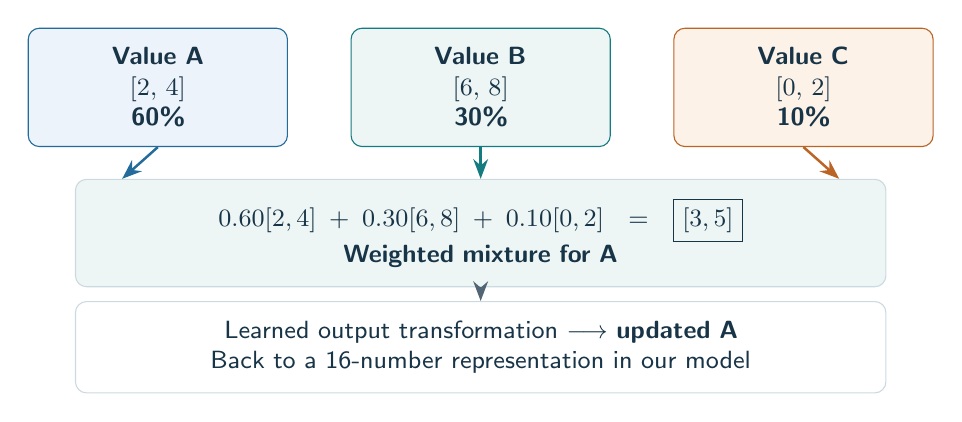
\begin{tikzpicture}[x=1cm,y=1cm]
\node[card,draw=blue,fill=paleblue,text width=2.8cm] (va) at (0,0) {\textbf{Value A}\\$[2,\,4]$\\\textbf{60\%}};
\node[card,draw=teal,fill=pale,text width=2.8cm] (vb) at (4.1,0) {\textbf{Value B}\\$[6,\,8]$\\\textbf{30\%}};
\node[card,draw=orange,fill=paleorange,text width=2.8cm] (vc) at (8.2,0) {\textbf{Value C}\\$[0,\,2]$\\\textbf{10\%}};
\node[card,fill=pale,text width=9.8cm,minimum height=1.05cm] (mix) at (4.1,-1.85) {$0.60[2,4]+0.30[6,8]+0.10[0,2]=\boxed{[3,5]}$\\\textbf{Weighted mixture for A}};
\draw[arr,blue] (va.south)--($(mix.north west)+(.6,0)$);
\draw[arr,teal] (vb.south)--(mix.north);
\draw[arr,orange] (vc.south)--($(mix.north east)+(-.6,0)$);
\node[card,text width=9.8cm,minimum height=.85cm] (out) at (4.1,-3.3) {Learned output transformation $\longrightarrow$ \textbf{updated A}\\Back to a 16-number representation in our model};
\draw[arr] (mix.south)--(out.north);
\end{tikzpicture}
\end{center}
\end{minipage}

\callout{\textbf{Say it simply:} ``Each headline compares itself with the group. Those scores determine how much information it takes from each headline, including itself. The weighted mixture becomes its updated representation.''}
\begin{minipage}[t]{.49\linewidth}
\textbf{Where do the rules come from?} Training errors adjust the query, key, value and output transformations. Attention weights are then recalculated for each input group.
\end{minipage}\hfill
\begin{minipage}[t]{.47\linewidth}
\textbf{What happens next?} A \emph{second} attention step uses market context to weight these updated vectors into a daily news summary. These are different weights from the ones above.
\end{minipage}
\vfill
{\scriptsize\color{slate}Within-bucket, single-head illustration of our plain self-attention path. These weights are illustrative, not measured relevance or causal importance. Interactions do not guarantee better forecasts.}

\newpage
\heading{The final MLP receives numerical summaries of market and news}
\textbf{Thursday example:} after Thursday's close, use the previous Friday, Monday, Tuesday, Wednesday and Thursday to predict whether \textbf{Friday closes higher than Thursday}. Assume no holidays.

\begin{center}
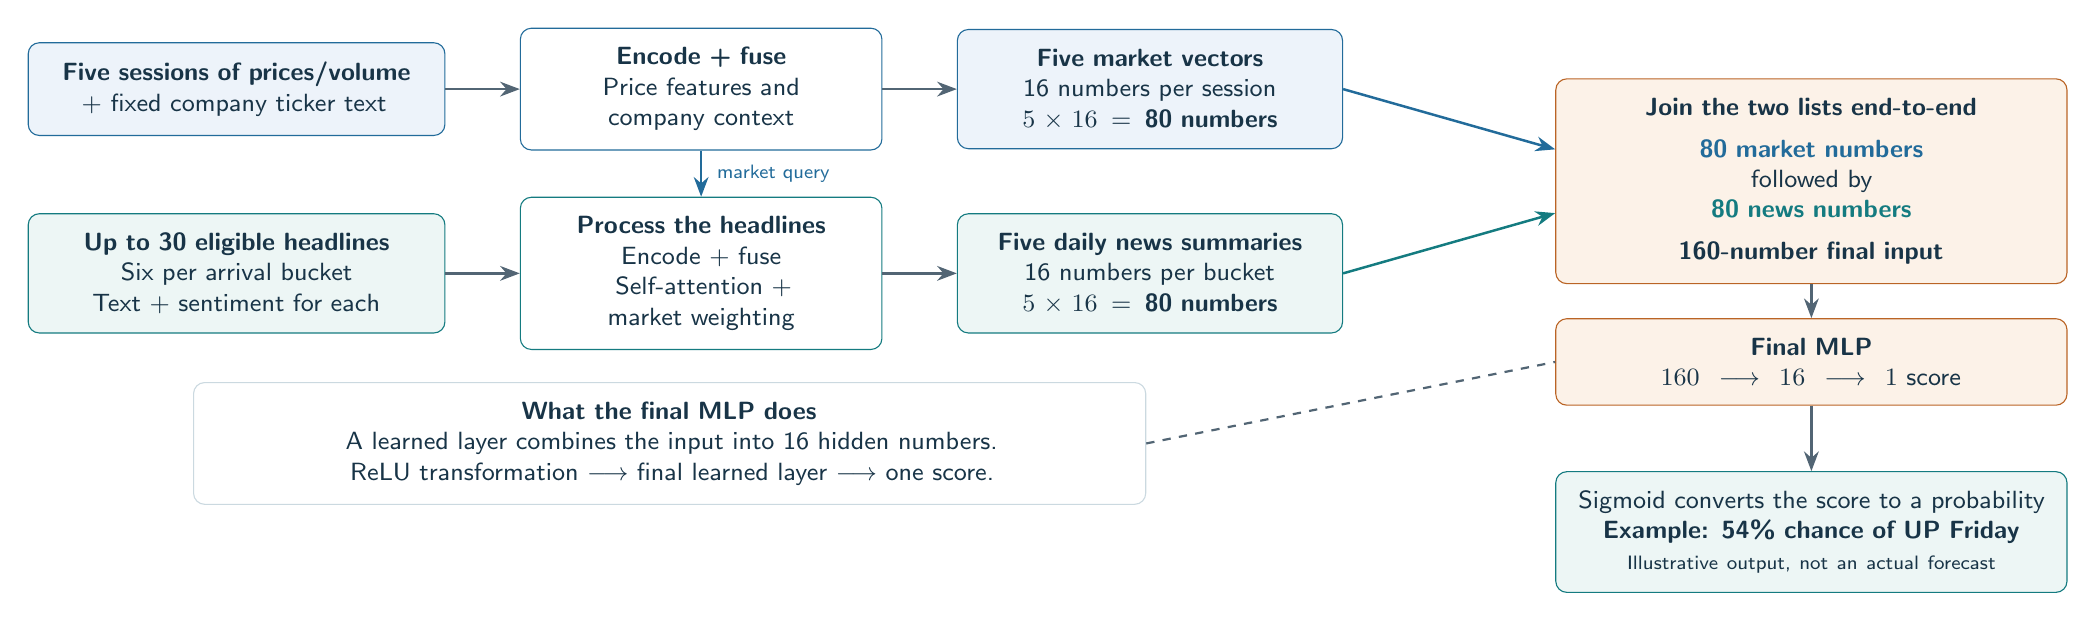
\begin{tikzpicture}[x=1cm,y=.9cm]
\node[card,draw=blue,fill=paleblue,text width=4.8cm,minimum height=1.15cm] (mi) at (0,0) {\textbf{Five sessions of prices/volume}\\+ fixed company ticker text};
\node[card,draw=blue,text width=4.1cm,minimum height=1.15cm] (me) at (5.9,0) {\textbf{Encode + fuse}\\Price features and company context};
\node[card,draw=blue,fill=paleblue,text width=4.4cm,minimum height=1.15cm] (mv) at (11.6,0) {\textbf{Five market vectors}\\16 numbers per session\\$5\times16=\textbf{80 numbers}$};
\draw[arr] (mi)--(me);\draw[arr] (me)--(mv);

\node[card,draw=teal,fill=pale,text width=4.8cm,minimum height=1.3cm] (ni) at (0,-2.6) {\textbf{Up to 30 eligible headlines}\\Six per arrival bucket\\Text + sentiment for each};
\node[card,draw=teal,text width=4.1cm,minimum height=1.3cm] (ne) at (5.9,-2.6) {\textbf{Process the headlines}\\Encode + fuse\\Self-attention + market weighting};
\node[card,draw=teal,fill=pale,text width=4.4cm,minimum height=1.3cm] (nv) at (11.6,-2.6) {\textbf{Five daily news summaries}\\16 numbers per bucket\\$5\times16=\textbf{80 numbers}$};
\draw[arr] (ni)--(ne);\draw[arr] (ne)--(nv);
\draw[arr,blue] (me.south)--(ne.north) node[midway,right,text=blue,font=\scriptsize,xshift=2pt] {market query};

\node[card,fill=paleorange,draw=orange,text width=6cm,minimum height=2.1cm] (join) at (20,-1.3) {\textbf{Join the two lists end-to-end}\\[4pt]\textcolor{blue}{\textbf{80 market numbers}}\\followed by\\\textcolor{teal}{\textbf{80 news numbers}}\\[4pt]\textbf{160-number final input}};
\draw[arr,blue] (mv.east)--($(join.west)+(0,.45)$);
\draw[arr,teal] (nv.east)--($(join.west)+(0,-.45)$);

\node[card,text width=11.6cm,minimum height=1.2cm] (inside) at (5.5,-5.0) {\textbf{What the final MLP does}\\A learned layer combines the input into 16 hidden numbers.\\ReLU transformation $\longrightarrow$ final learned layer $\longrightarrow$ one score.};
\node[card,fill=paleorange,draw=orange,text width=6cm,minimum height=.8cm] (mlp) at (20,-3.85) {\textbf{Final MLP}\\$160\longrightarrow16\longrightarrow1$ score};
\node[card,draw=teal,fill=pale,text width=6cm,minimum height=1.0cm] (pred) at (20,-6.25) {Sigmoid converts the score to a probability\\\textbf{Example: 54\% chance of UP Friday}\\{\scriptsize Illustrative output, not an actual forecast}};
\draw[arr] (join.south)--(mlp.north);\draw[arr] (mlp.south)--(pred.north);
\draw[link,dashed] (inside.east)--(mlp.west);
\end{tikzpicture}
\end{center}

\sub{FININ and our two versions: same idea, different news arrangement}
{\small
\begin{tabularx}{\linewidth}{@{}P{4cm}YYP{3.4cm}@{}}
\toprule
\textbf{Version} & \textbf{Market block received} & \textbf{News block received} & \textbf{Final input size}\\\midrule
FININ paper, Eq. 7 & Encoded market vector for each input day & Weighted news-summary vector for each input day & Depends on lookback and width\\
Our baseline (diagram above) & Five vectors: $5\times16=80$ & Five summaries: $5\times16=80$ & \textbf{160 numbers}\\
Our recent pooled/decay tests & Same five vectors: \textbf{80} & Pool the five buckets into \textbf{one 16-number summary} & \textbf{96 numbers}\\\bottomrule
\end{tabularx}
}
\callout{\textbf{Say it simply:} ``The MLP receives a long list of market numbers and summarized news numbers. Headline text, sentiment and attention weights have already shaped the news summary; they are not separate raw inputs to this final step.''}
{\small\textbf{Timing:} news must be eligible by Thursday's cutoff. Our date-based rule assumes availability from source date $D+2$; Tuesday-dated news can therefore enter Thursday's bucket. Exact historical availability remains uncertain.}
\vfill
{\scriptsize\color{slate}FININ market context describes the index; ours uses fixed company ticker context. Actual widths verified against local model code. Reference: \href{https://aclanthology.org/2024.findings-emnlp.189.pdf}{Wang, Cohen \& Ma (2024), Sections 4.1--4.3, Eq. 7}.}
\end{document}
